\chapter{Elastic collisions}
\label{elastic}\index{Elastic collisions}
Everything described here happens in the rest frame of the cell.
There are four processes that can happen:
\begin{enumerate}
\item $q\color{forest-green}q\color{black} 
  \rightarrow q\color{forest-green}q\color{black}$
\item $g\color{forest-green}q\color{black} 
  \rightarrow g\color{forest-green}q\color{black}$
\item $q\color{forest-green}g\color{black} 
  \rightarrow q\color{forest-green}g\color{black}$
\item $g\color{forest-green}g\color{black} 
  \rightarrow g\color{forest-green}g\color{black}$
\end{enumerate}
where $q$ can be a quark or anti-quark. The second parton is always the thermal one,
while the first is the jetty one. Fig. \ref{fig:feynmanelasitc} shows 
the processes in terms of Feynman diagrams.
\begin{figure}[htb]
  \begin{center}
    \includegraphics[width=16cm]{feynmanelastic.jpg}
    \caption{Elastic processes. Green lines indicate a thermal parton. 
      \label{fig:feynmanelasitc}}
  \end{center}
\end{figure}


\section{Total probabilities}
To determine whether in one time step $\Delta t$ an elastic collision
occurs for a gluon or a light quark, we use the transition rate
\begin{align}\label{transition}
 \frac{d\Gamma}{d\omega}~&(E,\omega,T)=\frac{d_k}{(2\pi)^3}\frac{1}{16\,E^2}\int_0^p dq \int_{\frac{q-\omega}{2}}^\infty dk\,\theta(q-|\omega|)\int_0^{2\pi}\frac{d\phi_{kq|pq}}{2\pi}|\mathcal{M}|^2 f(k,T)(1\pm f(k^\prime,T))\,,
\end{align}
integrate it over $\omega$ and multiply by the size of the time step $\Delta t$.
We choose a minimal $|\omega_{\rm min}|=0.05\,T$, where $T$ is the temperature.
The result $\int_{-\infty}^{-\omega_{\rm min}}\frac{d\Gamma}{d\omega} d\omega+\int_{\omega_{\rm min}}^{\infty}\frac{d\Gamma}{d\omega} d\omega$ is parametrized using a fit.

We use method B as described in Ref. \cite{Schenke:2009ik} 
to compute (\ref{transition}).

These total probabilities are stored in \\
#double Elastic::totalRate(double p, double T, double alpha_s, int Nf, int process)# \\
which reads #p# and #T# in units of GeV.

\section{Sampling the energy transfer}
\label{omegasampling}\index{Elastic collisions!energy transfer}
See\\

\begin{boxedverbatim}
double Elastic::findValuesRejection(double u, double T, double alpha_s, int Nf,
                                    Random *random, Import *import, int process)
\end{boxedverbatim}
~\\
~\\
Please not that #findValuesRejection# takes the energy #u# in units of the 
temperature #T# and also returns #omega# in units of the temperature.

In case #MARTINI# decides, according to the total probabilities described above, 
that a certain elastic process occurs, we go on and sample $\omega$, 
the zeroth component of the four-momentum transfer $Q=(\omega,\mathbf{q})$. 
That is done using \ref{transition} wihout integrating it over $\omega$.
In particular, we use the rejection method to sample the tabulated and 
interpolated rates (see #Import# {\bf reference here}).

For scattering with a thermal quark, we use the envelope function
\begin{equation}\label{omegaenvelope}
  f(\omega)=\alpha_s\frac{0.035 + 0.02 \alpha_s}{0.15 \sqrt{\omega^2}}
\end{equation}
for both positive and negative $\omega$. Note that it depends on $\alpha_s$.
For positive $\omega$, the integral of function \ref{omegaenvelope} 
from a minimal value $\omega_{\rm min}=0.05\,T$ up to $\omega = y$, is given by
\begin{equation}
  \frac{\alpha_s}{30}(7.+ 4.\alpha_s)(2.99573+\log(y))\,.
\end{equation}
For negative $\omega$, we have
\begin{equation}
  -0.133333 \alpha_s(1.75+\alpha_s)\log(-0.0833333*y)\,.
\end{equation}
These are both saved in\\ 
#double Elastic::area (double y, double alpha_s, int posNegSwitch, int process)#,\\ 
as well as those for the processes that involve a thermal gluon and use the envelope
\begin{equation}\label{omegaenvelope}
  f(\omega)=10\, \alpha_s\frac{0.035 + 0.02 \alpha_s}{\sqrt{\omega^2}}\,.
\end{equation}
These are for positive $\omega$
\begin{equation}
  0.05\,\alpha_s\,(7.+ 4.\,\alpha_s)(2.99573+\log(y))\,
\end{equation}
and for negative $\omega$
\begin{equation}
 -0.2\,\alpha_s\,(1.75+\alpha_s)\,\log(-0.0833333\,y)\,.
\end{equation}
The inverse of these integrals, e.g.
\begin{align}
  \tilde{\omega} &= \exp\left(\frac{-1.41428\,10^9\,\alpha_s - 8.08158\,10^8\,\alpha_s^2 + 2.02327\,10^9 \lambda}{\alpha_s\,(4.72097\,10^8 + 2.6977\,10^8\,\alpha_s)}\right)\,,
\end{align}
for $qq \rightarrow qq$ is the probability distribution of $\tilde{\omega}$, 
an auxiliary quantity. Here $\lambda$ is a uniformly distributed random variable, 
which is maximally the full area under the envelope, here:\\
$\lambda=$#random->genrand64_real1()*area(u,alpha_s,posNegSwitch,process)#\,, 
where #u#$=E$ is the energy of the jet.

Its value will be accepted, and assigned to $\omega$, if another uniformly 
distributed variable, say $x \in [0,1]$ is smaller than 
$\frac{d\Gamma}{d\omega}~(E,\tilde{\omega},T)/f(\tilde{\omega})$, 
where $f$ is the used envelope function, otherwise it will be rejected 
and another $\tilde{\omega}$ will be chosen, and the process starts over 
 - until an $\omega$ is accepted.

\section{Sampling the momentum transfer}
\index{Elastic collisions!momentum transfer}
See\\

\begin{boxedverbatim}
double Elastic::findValuesRejectionOmegaQ(double p, double omega, double T, 
                                          double alpha_s, int Nf, Random *random,
                                          Import *import, int process)
\end{boxedverbatim}
~\\~\\
Please note that #findValuesRejectionOmegaQ# takes the energy #u# and #omega# 
in units of the temperature #T#, and also returns #q# in units of the temperature.

To determine the transferred momentum for a given transferred energy $\omega$,
we sample the transition rate
\begin{align}\label{transitionq}
 \frac{d\Gamma}{d\omega\,dq}~&(E,\omega,q,T)=
 \frac{d_k}{(2\pi)^3}\frac{1}{16\,E^2} 
 \int_{\frac{q-\omega}{2}}^\infty dk\,\theta(q-|\omega|)
 \int_0^{2\pi}\frac{d\phi_{kq|pq}}{2\pi}|\mathcal{M}|^2 f(k,T)(1\pm f(k^\prime,T))\,,
\end{align}
which is just (\ref{transition}) without the integral over $q$, at the given $\omega$,
 as determined before (see Section \ref{omegasampling}).

Here we use two different methods to sample $q$. For $\omega<6\,T$, 
we use the rejection method with the envelope function
\begin{equation}
  f(q)=A\,\frac{q}{q^4+B}\,,
\end{equation}
where 
\begin{align}
  A &= (0.7+\alpha_s)\,0.0012\,(1000. + 40./\sqrt{\omega^2} + 10.\omega^4)\,\alpha_s\\
  B &= 2.\,\sqrt{\omega^2} + 0.01
\end{align} 
for processes 1 and 2 ($qq \rightarrow qq$ and $gq \rightarrow gq$), and
\begin{align}
  A &= (0.7+\alpha_s)\,0.0022\,(1000. + 40./\sqrt{\omega^2} + 10.\omega^4)\,\alpha_s\\
  B &= 2.\,\sqrt{\omega^2} + 0.002
\end{align} 
for processes 3 and 4 ($qg \rightarrow qg$ and $gg \rightarrow gg$).
Note again, that here the overall normalization of (\ref{transitionq}) does not matter.
It is only important for the total transition rate, when we determine the total 
probability for the process to happen. Hence, to sample $q$ (or $\omega$), we can 
neglect the factor of $9/4$ for the processes involving a thermal gluon.

The area under the envelope function up to $q=y$ is given by
\begin{equation}\label{areaq}
  F(y)=0.5\,A\,\frac{\arctan\left(\frac{y^2}{\sqrt{B}}\right)
    -\arctan(\frac{\omega^2}{\sqrt{B}})}{\sqrt{B}}
\end{equation}
with $A$ and $B$ as above. Note that we limited the integration to $q>\omega$.

Finally, we determine invert (\ref{areaq}) and get an equation for $\tilde{q}$
\begin{align}
 B^{0.25}\,\sqrt{\tan\left(\frac{2.\sqrt{B}\,x +A\,\arctan(\omega^2/\sqrt{B})}{A}\right)}\,,
\end{align}
where $x=#random->genrand64_real1()*areaOmegaQ(p,omega,alpha_s,process)#$
is a uniformly distributed random number on 
$[0,#areaOmegaQ(p,omega,alpha_s,process)#]=[0,F(\omega)]$ (see Eq.\ref{areaq}), where $p=E$ (the parton's energy)
is the maximal value for $\tilde{q}$.
Then we compare the ratio 
$$r=\frac{d\Gamma}{d\omega\,dq}(E,\omega,\tilde{q},T)/f(E,\omega,\tilde{q},T)$$ 
to a uniformly distributed random number $x$ and reject the value of
$\tilde{q}$ if $x > r$, otherwise we accept and the final result $q=\tilde{q}$ 
is passed to #MARTINI#.

For $6<\omega<60\,T$ we use a different envelope $$f(q)=A\,\exp(-0.5\,q)\,,$$ but the same principle method. 

For $\omega>60\,T$ we use Metropolis sampling.

\section{Determining the new $\vec{p}'$}
After we have sampled $\omega$, the transferred energy, and $q=|\mathbf{q}|$, we can 
determine the momentum vector $\mathbf{p^{\prime}}$, the final momentum of the 
parton after the elastic collision.
This is done in\\

\begin{boxedverbatim}
Vec4 Elastic::getNewMomentum(Vec4 vecpRest, double omega, double q, Random *random)
\end{boxedverbatim}
~\\~\\
This function takes the old momentum vector $\mathbf{p}=$ #vecpRest# 
(well, the three-vector contained in #vecpRest#), $\omega$, and $q$ as arguments
and from them finds a new $\mathbf{p^\prime}$.

Using the angle between $\mathbf{p}$ and $\mathbf{q}$, $\theta_{pq}$,
we can separate $\mathbf{q}$
into $q_\parallel$ and $q_\perp$, which are the components parallel and perpendicular
to $\mathbf{p}$, respectively.
With
\begin{equation}
  \cos(\theta_{pq}) = \frac{p^2+q^2-(p-\omega)^2}{2\,p\,q}\,,
\end{equation}
we find
\begin{align}
  q_\perp &= q\,\sin(\theta_{pq}) = q\,\sqrt{1-\cos^2(\theta_{pq})}\\
  q_\parallel &= q\,\cos(\theta_{pq})
\end{align}
Then, using the cross product of $\mathbf{p}$ with $\mathbf{e}_x$ or $\mathbf{e}_y$,
depending whether $\mathbf{p}$ points more into the $y$ or the $x$ direction, 
we find a vector perpendicular to $\mathbf{p}$.
This vector, normalized to 1, is taken time $q_\perp$ 
and then subtracted from $\mathbf{p}$. 
Finally, take $\mathbf{e}_\parallel=\mathbf{p}/p$, multiply it by $q_\parallel$ and
subtract it from $\mathbf{p}$ as well.

This way we find
\begin{equation}
  \mathbf{\tilde{p}}=\mathbf{p}-\mathbf{q}=\mathbf{p}-q_\perp\,\mathbf{e}_\perp
  -q_\parallel\,\mathbf{e}_\parallel\,.
\end{equation}

Since we want the new vector $\mathbf{p^\prime}$ to point in a direction with arbitrary azimuthal angle
around $\mathbf{p}$, we rotate $\mathbf{\tilde{p}}$ around $\mathbf{p}$ by a 
random angle $\phi=2\,\pi\,#random->genrand64_real1()#$.
This is done using the rotation matrix
\[ \mathcal{M}= \left( \begin{array}{lll}
x^2\,(1-\cos(\phi))+\cos(\phi) 
&x\,y\,(1-\cos(\phi))+z\,\sin(\phi) 
&x\,z\,(1-\cos(\phi))-y\,\sin(\phi) \\
y\,x\,(1-\cos(\phi))-z\,\sin(\phi) 
&y^2\,(1-\cos(\phi))+\cos(\phi) 
&y\,z\,(1-\cos(\phi))+x\,\sin(\phi) \\
z\,x\,(1-\cos(\phi))+y\,\sin(\phi) 
&z\,y\,(1-\cos(\phi))-x\,\sin(\phi) 
&z^2\,(1-\cos(\phi))+\cos(\phi) \end{array} \right)\,,\]
where $x=p_x/p$, $y=p_y/p$, and $z=p_z/p$. So finally we have
\begin{equation}
  \mathbf{p^\prime} = \mathcal{M}\cdot \mathbf{\tilde{p}}\,,
\end{equation}
which concludes this section.

\section{Conversion processes}
\label{conversion}
We include conversion via Compton and annihilation processes. Special care has to be taken 
about the color indices of the partons. E.g., when a quark is converted to a gluon we have
to add an aditional color line which has to be connected to another gluon (a thermal one),
which again has to have its other color index connected to another thermal parton (we always
use a quark for that one to end adding more connected thermal partons - that is fine because
it will only change the low momentum part of the hadronization).
Fig. \ref{fig:quarkConv} shows how the color lines are connected and the grey blobs are 
the thermal partons that are sampled from Fermi or Bose distributions at the present 
temperature. The momentum of the hard parton is not changed, as the momentum transfer 
is typically very small.
\begin{figure}[htb]
  \begin{center}
    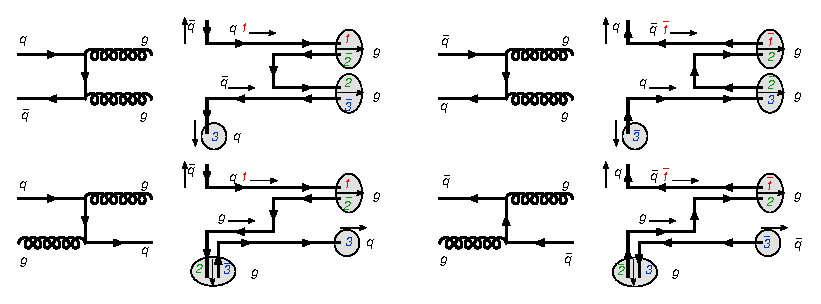
\includegraphics[width=16cm]{quarkConversion1}
    \caption{$q\rightarrow g$ and $\bar{q}\rightarrow g$ Feynman diagrams on the left and corresponding color lines
    on the right. The upper part of each diagram represents the hard partons, the lower part 
the thermal ones.
      \label{fig:quarkConv}}
  \end{center}
\end{figure}

Processes that convert a gluon into a quark or anti-quark are treated analogously.




%%% Local Variables: 
%%% mode: latex
%%% TeX-master: "manual"
%%% End: 
